\chapter{Estado del Arte\label{sec:estado_del_arte}}
En este apartado se analiza el contexto y la situación de las tecnologías involucradas en este proyecto. Por ello, en este capitulo trataremos la situación en la que se encuentran los datos abiertos, como los aquí utilizados, en cuanto a su acceso y beneficios. 

Además también realizaremos un análisis sobre la situación actual del \textit{big data}, las herramientas disponibles para crear sistemas de este tipo y, en especial, \textit{Apache Spark}, \textit{Apache Hadoop} y \textit{Apache Parquet}, que han sido las utilizadas para la implementación de los sistemas diseñados.

\section{Open data}

En este proyecto, los datos que se van a utilizar para hacer el procesamiento y las consultas es un fichero que contiene todos los viajes de taxis registrados en 2013 en la ciudad de Nueva York. Estos están disponibles de forma totalmente abierta en la página del ``Grand Challenge'' del \gls{DEBS} \cite{grandChallenge}. Sin embargo, estos datos pasaron a estar disponibles gracias al esfuerzo Chris Whong, que tuvo que realizar una petición del tipo \gls{FOIL} a las autoridades neoyorquinas para obtenerlos.

Este tipo de datos que está disponible de forma libre para todo el mundo, sin restricciones de ningún tipo, ya sean derechos de autor, patentes o cualquier otro mecanismo de control es conocidos como datos abiertos u open data, en inglés. Estos datos podrán ser utilizados y redistribuidos de forma libre por cualquier persona \cite{opendata}.

Aunque el término estaba definido desde el siglo pasado, en 1958 se crea la primera base de datos abiertos para la ciencia, el \gls{WDC} \cite{wdc}, ha sido con el proceso de digitalización de la sociedad y el  reciente auge de las herramientas \textit{big data} cuando más proliferación ha habido de estos movimientos.

Actualmente, un gran número de organismos gubernamentales y no gubernamentales tienen plataformas de acceso a datos abiertos sobres diferentes aspectos de la sociedad, como datos demográficos o económicos. Así podemos encontrar datos globales, como en el portal de datos la \gls{ONU} \cite{onudata}, a datos locales, como en el portal de datos abiertos de la ciudad de Madrid \cite{datosMadrid}.

Como se puede apreciar en la figura \ref{fig:opendata} el crecimiento del número de APIs para el acceso a datos ha aumentado de una forma importante desde 2006. También se puede observar como grandes países se han ido comprometiendo a liberar datos abiertos sobre diferentes asuntos de estado.

\begin{figure}[htp!]
\centering
\caption{Número de API de datos disponibles con respecto al tiempo y compromisos de abrir los datos de diferentes países del mundo \cite{graphdata}}
\label{fig:opendata}
\vspace{5pt}
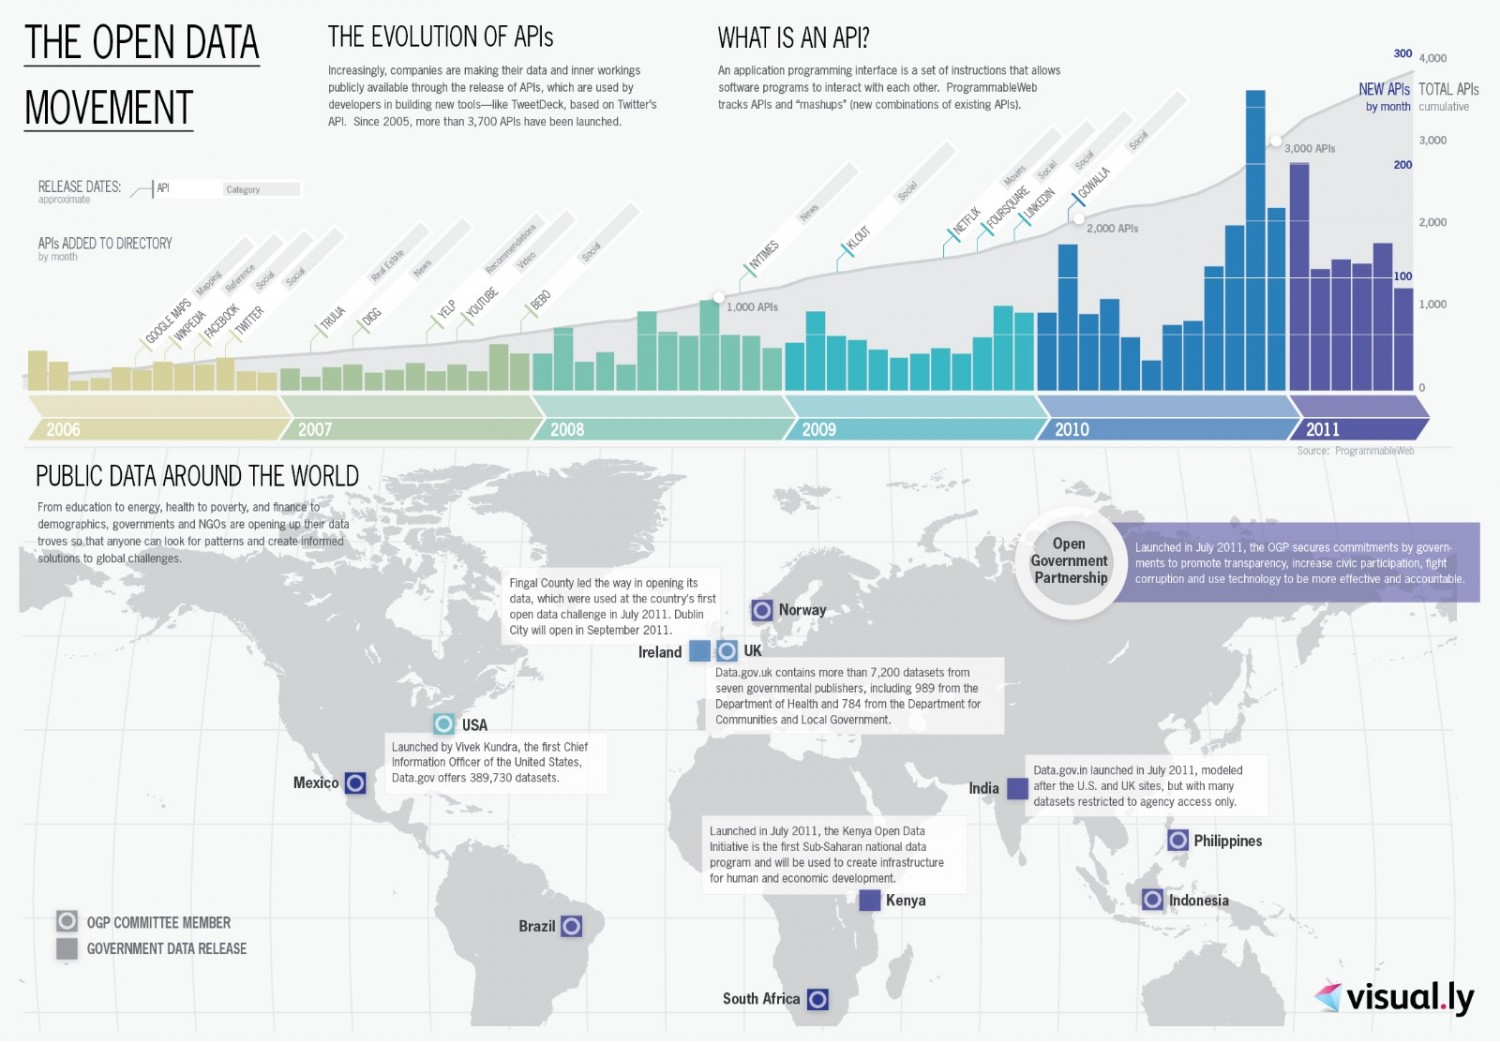
\includegraphics[scale=0.3]{graphics/opendata}
\end{figure}


Se estima que la apertura de datos, solo en Estados Unidos, puede generar entre 3 y 5 billones de dólares \cite{revenueOpenData}. El principal motivo es el gran potencial económico que puede suponer, ya que se podría aumentar la eficiencia en diferentes aspectos de la sociedad, como en la sanidad y educación, además, crearía nuevos servicios y productos, que irían acompañados de puestos de trabajo, y podrían mejorar la percepción para las personas sobre el mundo en general al aumentar la transparencia de la información.

Por otro lado en Europa, otros estudios prevén que el uso de datos abiertos reportará un ahorro de más de 1.7 billones de euros a las administraciones públicas, reducirá en un 16\% la energía consumida y el tiempo de espera en las carreteras. Aparte, indica que las compañías que siguen una filosofía de datos abiertos aumentan su valor en mayor medida que otras que no los abren \cite{valueOpenData}.

Por tanto, se espera que en el futuro cercano más y más países y organizaciones se sumen a estas iniciativas de apertura de datos y, que, los países que ya están participando en ellas, mejoren la calidad de la información que suministran, cuyos formatos, en ocasiones, no pueden ser utilizados sin una transformación a otros adecuados para la lectura por las máquinas.

\begin{figure}[htp!]
\centering
\caption{Valor potencial de los datos abiertos en billones de dólares en Estados Unidos}
\label{fig:revenue}
\vspace{5pt}
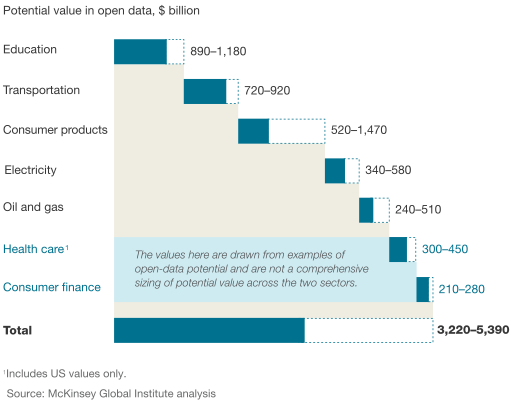
\includegraphics[scale=0.8]{graphics/revenue}
\end{figure}

\newpage
\section{Big Data}
\subsection{Introducción}
El término \textit{big data} es relativamente reciente, su primera aparición parece datar de 1989 cuando Erik Larson lo utilizó en una artículo para la revista Harper's, aunque, se creé que se definió como tal en los años noventa durante las charlas que daba John Mashey, científico jefe de Silicon Graphics, donde explicaba el término para vener sus productos, como se puede ver en presentaciones suyas de 1998 \cite{originbd}.

Sin embargo, los pilares en los que se basa el \textit{big data} no son nada nuevos. Los seres humanos nos hemos caracterizado por la idea de almacenar toda la información posible para crear una base de datos en continúa expansión que pueda ser analizada y de donde se extraiga conocimiento valioso para la humanidad.

Ya en el año 18000 \gls{AC}, había tribus paleolíticas que mediante muescas en palos y huesos hacían seguimientos de las reservas de suministros y de las actividades comerciales, permitiendo hacer predicciones sobre la duración de los alimentos almacenados. También, sobre el año 2400 \gls{AC} surge el ábaco en Babilonia que permitía realizar cálculos.

Como ejemplo de primer almacén de datos, tenemos a la Biblioteca Real de Alejandría, que fue la colección de conocimiento del antiguo mundo. Como primer ejemplo que definió el término ``Business intelligence'', contamos con el banquero Henry Furnese que utilizó en 1985 los datos recolectados de su negocio para obtener una ventaja competitiva frente a sus adversarios.

Pero es durante la segunda mitad del siglo XX y el XXI donde se produce los avances que han permitido llegar a la realidad actual. Hitos como el desarrollo de la computación, los sistemas de almacenamiento digital e Internet y las conexiones inalámbricas han sido las que han permitido crear y almacenar grandes cantidades de datos, unas cantidades que crecen exponencialmente con el tiempo.

\subsection{Definición \label{defBigData}}
Si buscamos la definición de \textit{big data} en Internet podemos encontrar diversas versiones de la misma \cite{ayuso}, algunas más correctas y otras menos, pero no existe un consenso claro sobre el término. Sin embargo, la agencia de la \gls{ONU} encargada de las tecnologías de la  información, creadora del primer estándar \textit{big data} lo define como un paradigma que permite la recolección, almacenamiento, manejo, análisis y visualización de extensos conjuntos de datos, con características heterogéneas y con restricciones de tiempo cercanas al tiempo real \cite{estandar}. 

Otro aspecto que ejemplifica estos cambios en la definición del concepto se puede apreciar en la conocida forma de describir el \textit{big data}, las V's. Estas comenzaron siendo tres \cite{ayuso}, para pasar a ser 4 \cite{4v} y, luego, 5 \cite{monse}, 7 \cite{soriano} e, incluso, 10. En la figura \ref{lasv} se puede apreciar como ha sido este proceso a lo largo del tiempo.

\begin{figure}[htp!]
	\centering
	\caption{Evolución de las V's que definen el \textit{big data} a lo largo del tiempo \cite{fotoV}}
	\label{lasv}
	\vspace{5pt}
	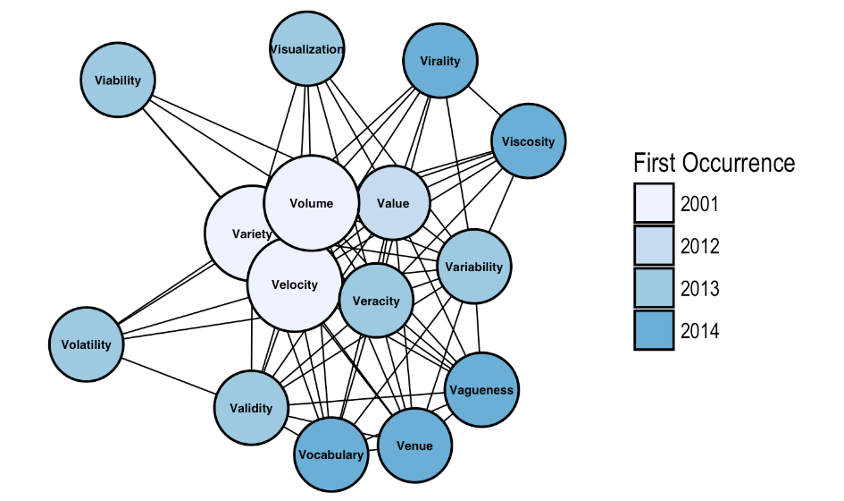
\includegraphics[scale=0.5]{graphics/lasv}
\end{figure}

Aunque, igual que en el caso de la definición, el número de V's variará dependiendo del experto al que consultes, podemos establecer cuatro aspectos básicos de un sistema para que este sea considerado \textit{big data}. Estos son:

\begin{itemize}
\item \textbf{Volumen:} Referido como al tamaño y la cantidad de los datos, aunque no existe un límite establecido ya que estas cantidades cada vez aumentan a un mayor ritmo.
\item \textbf{Velocidad:} Referido a la rapidez con la que se accede a los datos. Lo que se busca en un análisis en tiempo real.
\item \textbf{Variedad:} Referido al número de fuentes diferentes de donde provienen los datos. Los sistemas \textit{big data} tienen que poder procesar datos de diversos orígenes y estructuras.
\item \textbf{Veracidad:} Referido a la certeza de que los datos contenidos en el sistema son reales. Un sistema \textit{big data} debe procurar mantener a cero la información no veraz a razón de no perder eficiencia.
\end{itemize}

\subsection{Propósitos}
Muchas grandes compañías del sector tecnológico llevan años usando herramientas \textit{big data} para mejorar su negocio, compañías pioneras en este campo como Google y Yahoo que desarrollaron primeras versiones de esta tecnología buscando mejorar el resultado de sus buscadores.

Como ya se ha comentado anteriormente, las posibles aplicaciones de estas herramientas son infinitas. En general, disponer de un conjunto de datos que contengan información sobre situaciones pasadas o sobre sucesos y elementos que puedan influenciar un proceso es beneficioso para saber como actuar de la forma más correcta posible.

En general, se pueden encontrar cuatro tipos de usar herramientas \textit{big data} \cite{tipoAnalisis}. Por un lado, podemos encontrar el análisis prescriptivo, que es el más valioso y menos usado, que consiste la utilización de los datos para encontrar posibles caminos de actuación que permitan anticiparse al futuro y obtener ventaja. Un caso donde se está empezando a utilizar este tipo de análisis es en los sistemas de salud, donde conociendo los datos de un grupo, se pueden encontrar patrones para atajar enfermedades de la forma más efectiva.

Otro tipo de análisis es el predictivo, donde se busca detectar patrones que hayan ocurrido en el pasado para predecir el futuro. Este, está siendo especialmente utilizado en los procesos de venta, por ejemplo, para ajustar los precios en base a la oferta y la demanda, así como para preparar los ``stocks'' de los productos.

El análisis de diagnóstico es aquel que busca determinar porque se ha producido algún suceso, usando para ello los datos relacionados con el evento. Este es especialmente utilizado en marketing, para entender el efecto que han tenido las campañas, pero, también en sistemas de software, para conocer el motivo del error y poder evitar situaciones similares en el futuro.

Finalmente, el análisis descriptivo o minería de datos, que busca información valiosa entre todos los datos almacenados. Un ejemplo de este tipo de análisis se da en el estudio de los riesgos al ofrecer un crédito, donde se puede buscar en el pasado financiero del cliente datos que puedan describir la capacidad económica del mismo.

\subsection{Visión de negocio y futuro}
La amplias posibilidades que las herramientas \textit{big data} ofrecen junto con el conocido éxito de empresas y su, cada vez, más sencilla implementación está haciendo que cada vez más y más negocios implementen estas tecnologías.

El ``landscape'' también ha ido creciendo durante estos últimos años, debido al auge de estas tecnologías, haciendo que las herramientas y arquitecturas disponibles haya aumentado, disponiéndose de un amplio abanico de opciones que se adaptan a todo tipos de datos y análisis. En la figura \ref{landscape} se puede observar el panorama actual.

\begin{figure}[htp!]
	\centering
	\caption{Panorama de las tecnologías \textit{big data} en 2017 \cite{landscape}}
	\label{landscape}
	\vspace{5pt}
	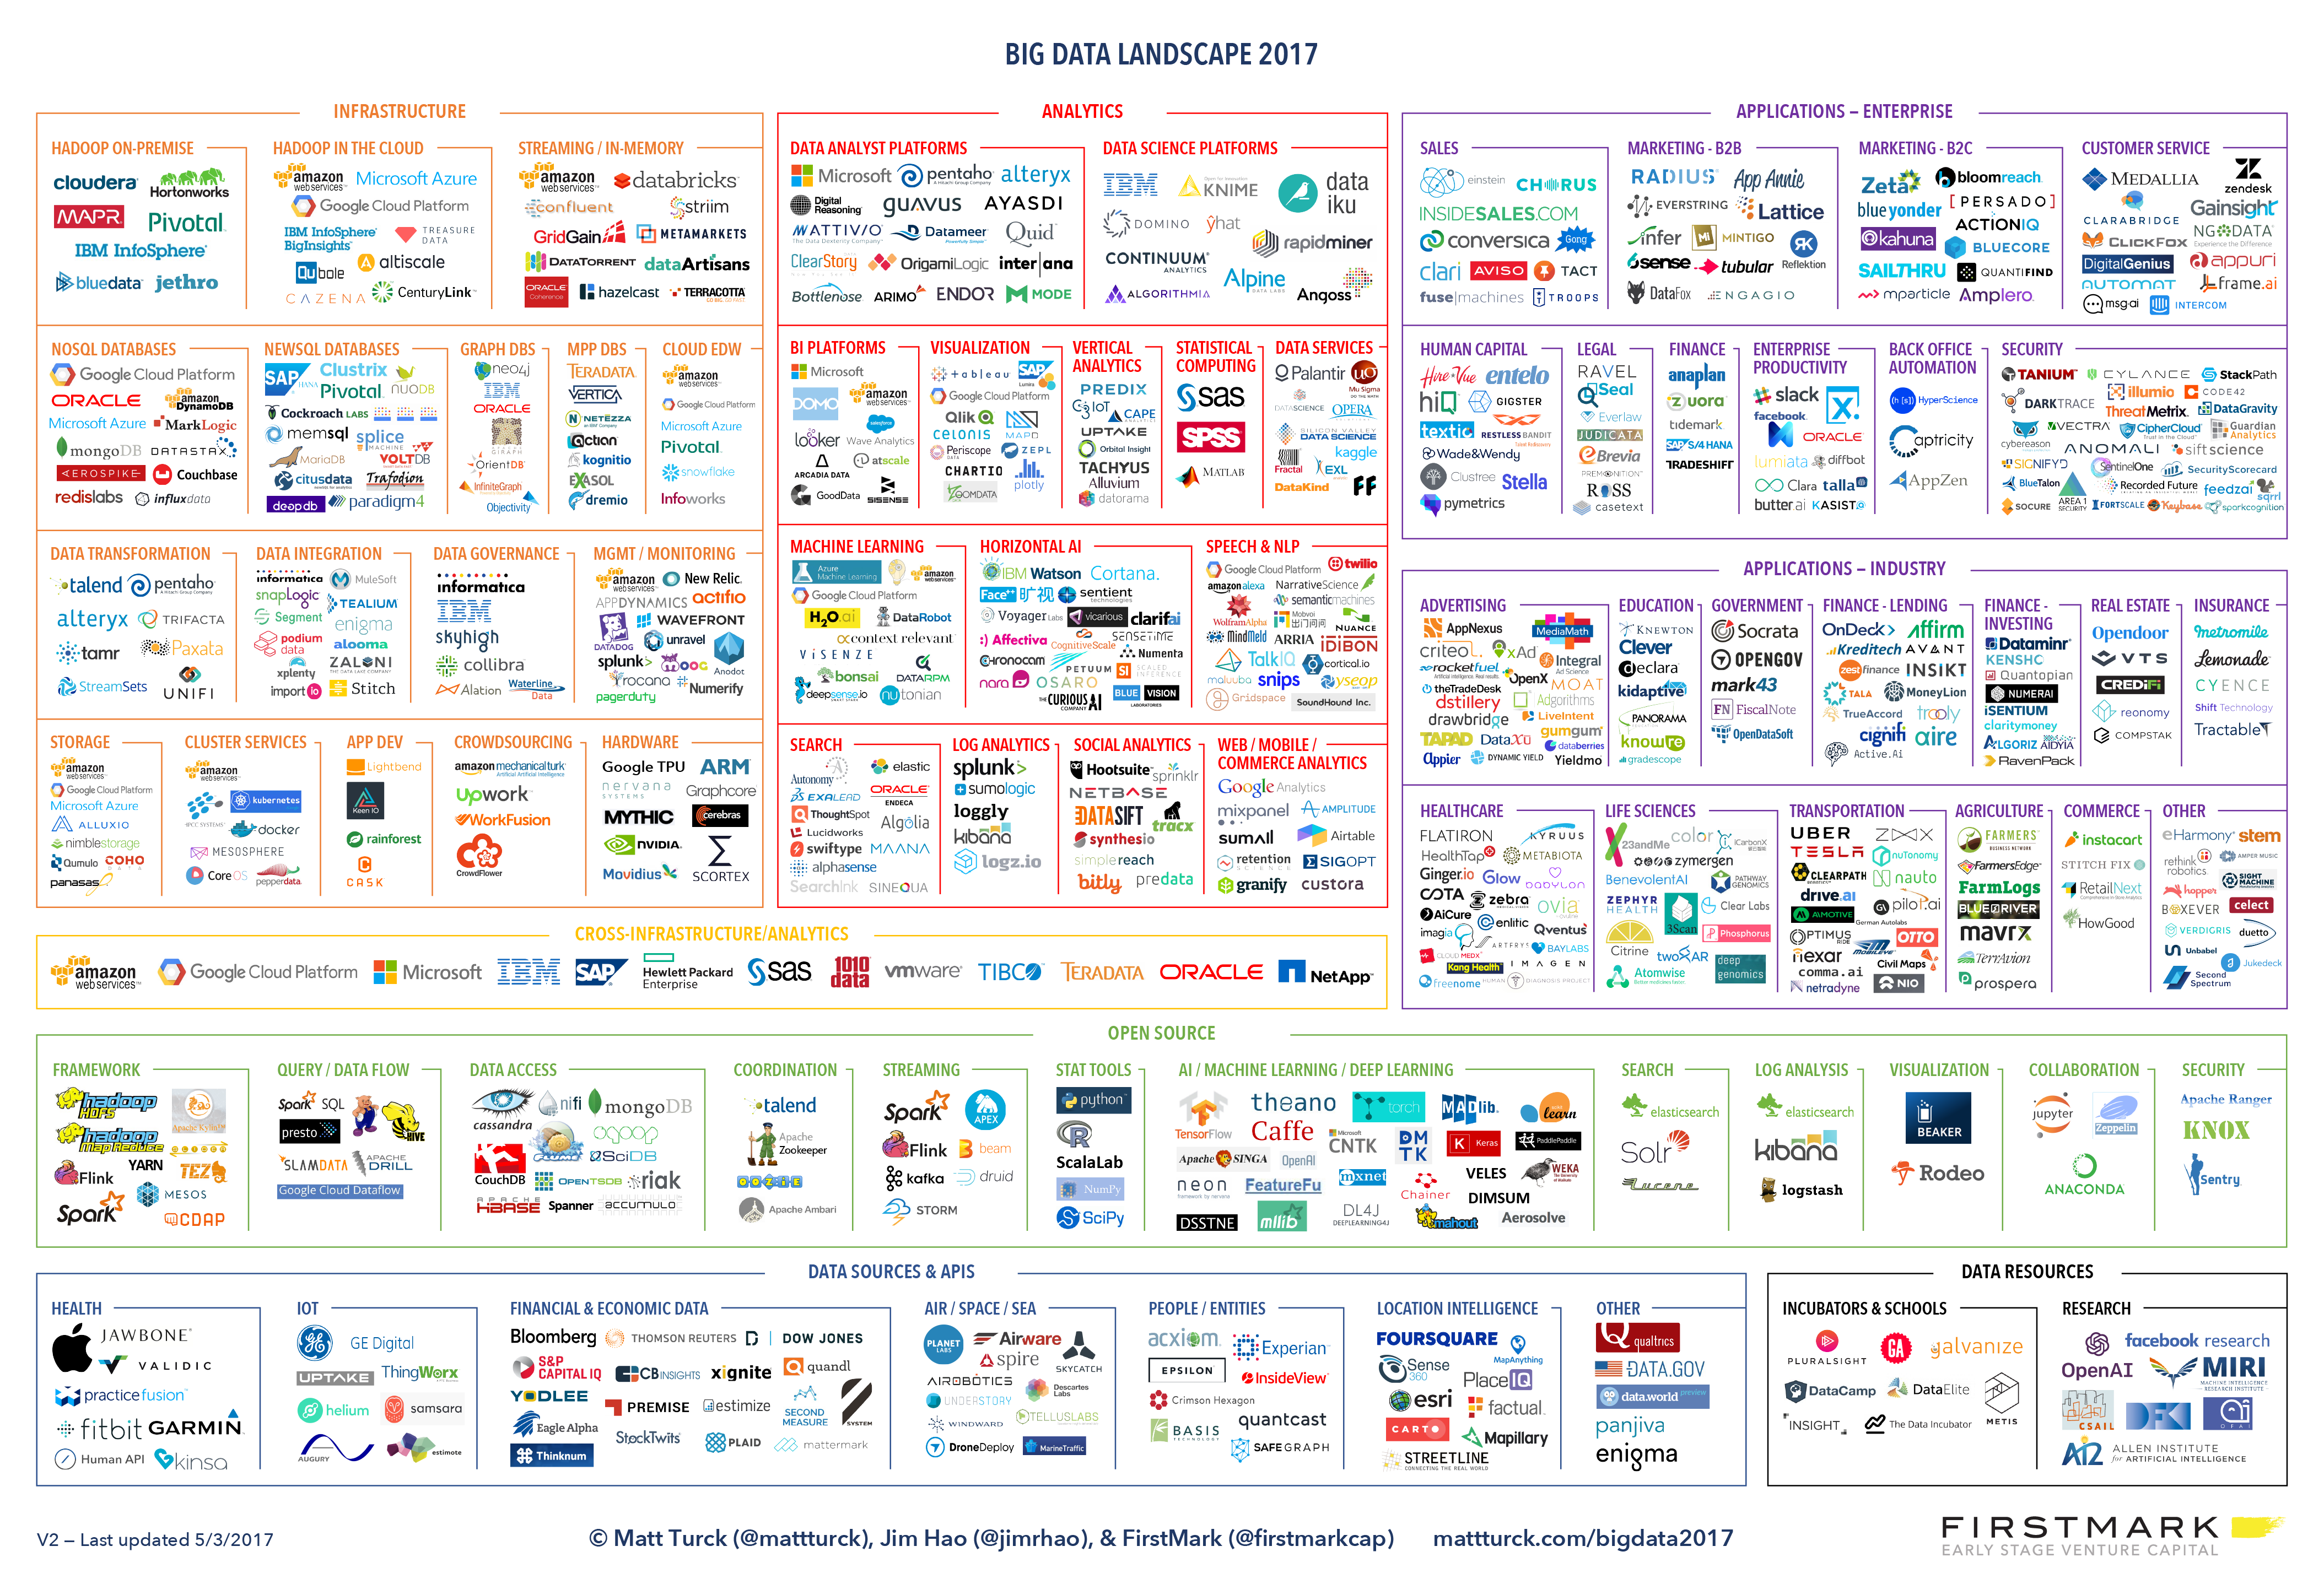
\includegraphics[scale=0.22]{graphics/landscape}
\end{figure}

Una de las características de este paradigma tecnológico es la naturaleza abierta de las herramientas, donde las más usadas son de código abierto y han surgido del resultado de la colaboración de diferentes empresas u organizaciones. Librerías como \textit{Apache Hadoop} \cite{hadoop} o \textit{Apache Spark} \cite{spark}, bases de datos como \textit{Apache Cassandra} \cite{cassandra} o \textit{MongoDB} \cite{mongo} y herramientas de análisis como \textit{SciPy} \cite{scipy} son de uso libre y no requieren de pago de licencias.

Esto ha hecho surgir empresas que se encargan de establecer y mantener un sistema \textit{big data}, es decir, ha permitido a los negocios externalizar este proceso, ahorrándose el presupuesto del diseño y la implantación de estos sistemas. Empresas como Hortonworks \cite{horton}, Cloudera \cite{cloudera} o Databricks \cite{databricks}, ofrecen sistemas de análisis de datos a empresas que utilizan las herramientas mentadas anteriormente, centrando su negocio en el cobro por el uso de recursos computacionales y el servicio técnico.

A este tipo de servicio que ofrecen estos negocios se les conoce como \gls{BDaaS} y se definen como servicios en la nube que permiten al usuario la capacidad de recoger, almacenar, analizar, visualizar y manejar los datos usando \textit{big data}.

El futuro del \textit{big data} parece prometedor, como se puede apreciar en la figura \ref{forecast}, proyectándose un crecimiento del 14.4\% anual en los ingresos generados por el \textit{big data}, pasando de los 18 billones de dólares en 2014 a los 92 en 2022. En general, las estadísticas de crecimiento son muy favorables para este sector tecnológico, con predicciones de entre el 4\% al 15\% \cite{forecast}.

Sin embargo, las tecnologías \textit{big data} no solo mejorarán los resultados económicos de las empresas. Estas, influirán directamente en los usuarios, mejorando las relaciones de estos con los servicios, principalmente, mediante la personalización de estos en base al cliente. También aumentarán la transparencia, al disponerse de más datos, permitiendo al usuario tener más conocimiento sobre las opciones disponibles.

\begin{figure}[htp!]
	\centering
	\caption{Proyección de los ingresos del \textit{big data}  \cite{forecast}}
	\label{forecast}
	\vspace{5pt}
	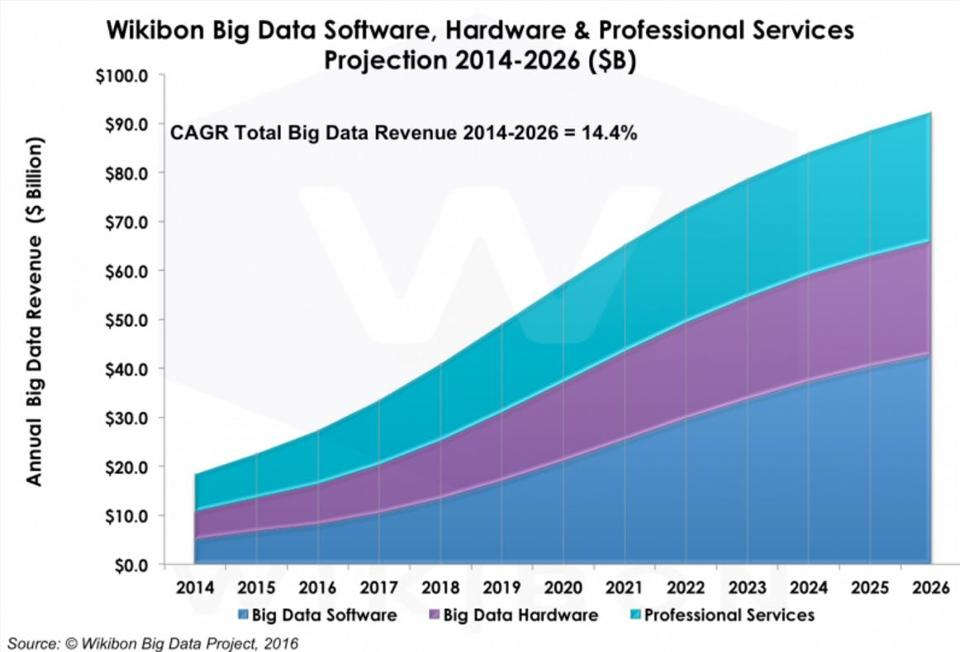
\includegraphics[scale=0.5]{graphics/forecast}
\end{figure}

\section{Sistemas distribuidos}
La computación distribuida es un modelo de computación que consiste en la conexión de diferentes máquinas, que pueden estar en localizaciones físicas distintas, con el fin de realizar tareas en un tiempo menor del que necesitaría una sola máquina. Es decir, un sistema distribuido es una red de equipos autónomos que se comunican entre ellos para conseguir un objetivo. Estos son independientes en el sentido que no comparten memoria o procesadores físicamente \cite{computacionDistribuidad}.

Estos ordenadores se comunican entre ellos por ``mensajes'' que son fragmentos de información que se intercambian por la red. Estos mensajes sirven para ordenar diferentes tareas con argumentos particulares, para enviar y recibir paquetes de datos o para mandar ordenar comportamientos específicos de otros ordenadores. Estas máquinas pueden tener diferentes roles dentro del sistema, dependiendo de su objetivo. 

\begin{figure}[htp!]
	\centering
	\caption{Esquema computación distribuida \cite{fotodistribuida}}
	\label{distribuida}
	\vspace{5pt}
	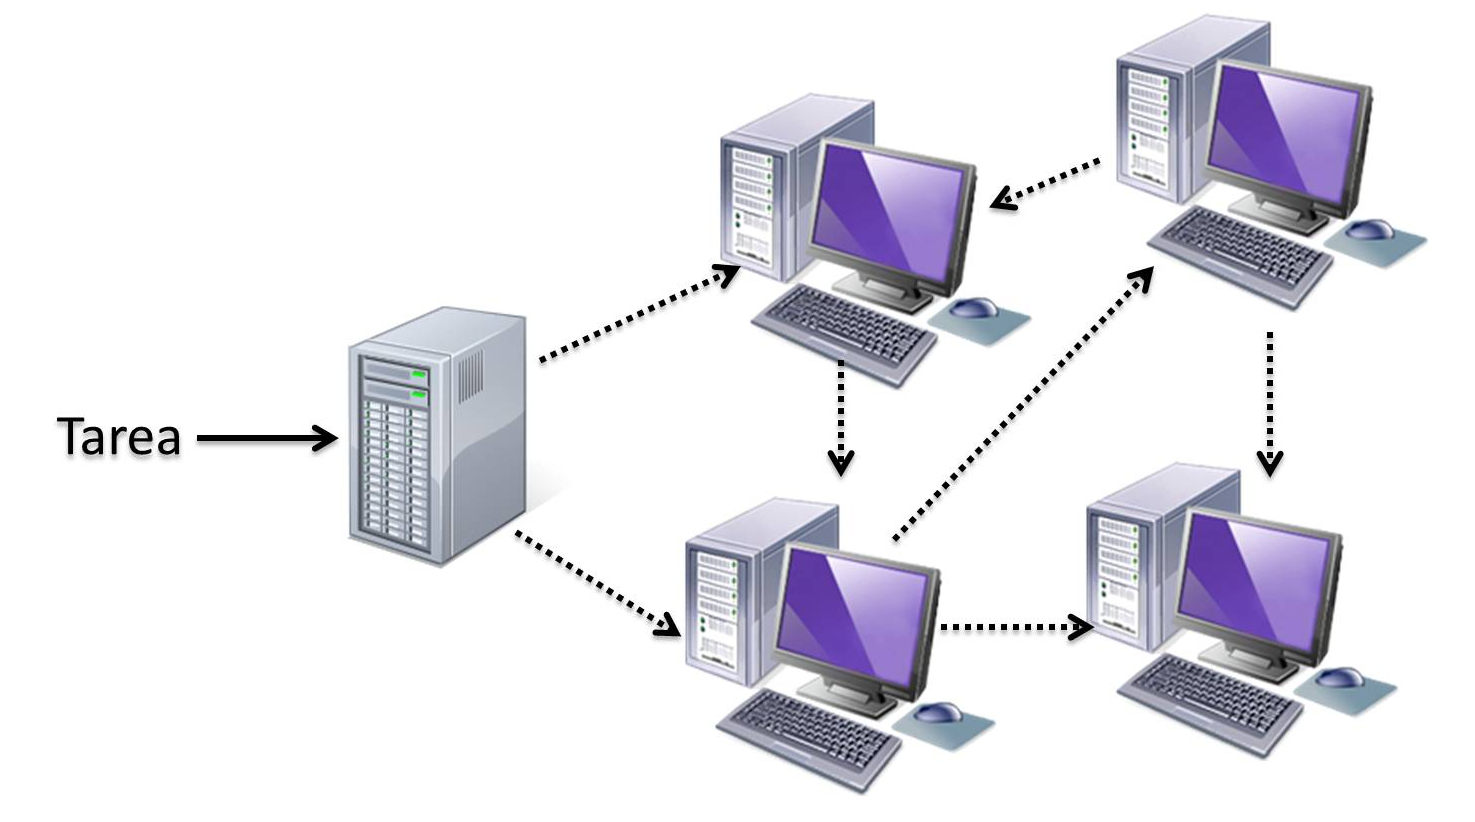
\includegraphics[scale=0.3]{graphics/computaciondistribuida}
\end{figure}

Las ventajas que ofrece este tipo de computación son \cite{sistDistTeoria}:

\begin{itemize}
\item \textbf{Compartición de recursos:} Este modelo de computación permite que las máquinas compartan recursos de hardware al estar conectadas en red.

\item \textbf{Escalabilidad:} Gracias a la capacidad de compartir recursos, nuevos sistemas pueden ser añadidos a la red y aumentar la capacidad del conjunto.

\item \textbf{Tolerancia a fallos:} Al contarse con varias máquinas, la caída de alguna de ellas de la red no será crítico, permitiendo la continuidad del sistema.

\item \textbf{Concurrencia:} Este modelo permite que se ejecuten varios procesos al mismo tiempo dentro de la red.

\item \textbf{Variedad:} Se pueden incorporar máquinas con diferente hardware y software debido al uso de protocolos estándar.
\end{itemize}

A pesar de estas ventajas, también cuenta con inconvenientes como los siguientes:

\begin{itemize}
\item \textbf{Complejidad:} Por el hecho de que se cuenta con varias máquinas, la organización y control de estos sistemas es más complicado que el de una sola máquina.

\item \textbf{Seguridad:} Debido a que existen conexiones remotas que conectan a los equipos del sistema, se puede dar el caso de escuchas e interceptación de mensajes.

\item \textbf{Disparidad en el comportamiento:} Se puede dar el caso de obtención de resultados diferentes dependiendo de las condiciones.
\end{itemize}

\subsection{Configuraciones}
Existen dos arquitecturas predominantes para la creación de sistemas distribuidos, la configuración cliente-servidor y la ``peer-to-peer''.

\subsubsection{Cliente-servidor}
La arquitectura cliente-servidor es una forma de ofrecer servicios desde una fuente central, es decir, existe un solo servidor a los que múltiples clientes se conectan para consumir sus productos. 

\begin{figure}[htp!]
	\centering
	\caption{Esquema cliente-servidor  \cite{computacionDistribuidad}}
	\label{clientserver}
	\vspace{5pt}
	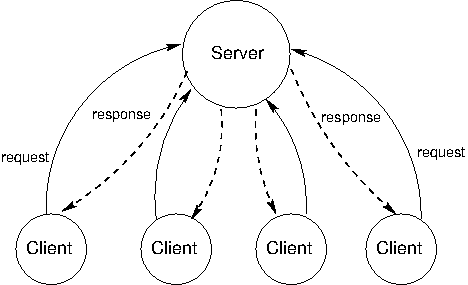
\includegraphics[scale=0.6]{graphics/clientserver}
\end{figure}

En este tipo los roles de los equipos son diferentes, mientras que el servidor es responder a las peticiones de los clientes, el trabajo de los clientes es usar los datos recibidos desde el servidor para realizar alguna tarea.

Internet es un ejemplo muy importante de este tipo de arquitectura ya que esta basada en ella, donde el servidor es una máquina que ofrece la página web a los sistemas que se conectan con ella. Sin embargo este sistema tiene dos importantes inconvenientes, por un lado, si se cae el servidor se paraliza el servicio totalmente. Por otro, este modelo no tiene capacidad de escalar, por lo que cuando hay muchos clientes conectados el rendimiento disminuye.

\subsubsection{Peer-to-peer}
Son aquellos sistemas distribuidos en los que el trabajo está dividido entre todos los componentes del sistema. Todos las máquinas envían y reciben datos y aportan capacidad de computación y memoria al sistema, siendo este más potente cuanto más integrantes tenga la arquitectura.

\begin{figure}[htp!]
	\centering
	\caption{Esquema peer-to-peer \cite{peertopeer}}
	\label{peertopeer}
	\vspace{5pt}
	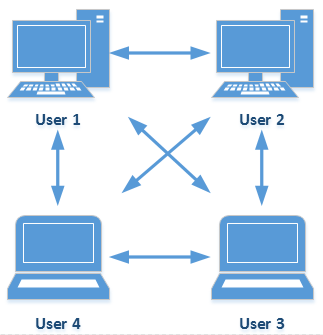
\includegraphics[scale=0.6]{graphics/peertopeer}
\end{figure}

La división del trabajo entre todos las máquinas es el aspecto clave de esta arquitectura y, para mantenerla, mantener un comunicación fiable es básico. Por ello, para asegurar que los mensajes llegan entre los componentes, la red de un sistema peer-to-peer es estructurada y todos los nodos del mismo tienen que procurar en tener suficiente información de la misma para mantenerlo.

Existen variaciones de este sistema donde hay elementos que se preocupan de mantener la conexión entre todos los equipos de la red, de controlar la información del sistema y proporcionarla y organizar las tareas del conjunto. Este tipo de sistema es el que utilizaremos en este proyecto, donde habrá un maestro que organizará las tareas y los esclavos que realizarán el procesamiento.

Las aplicaciones más comunes de este tipo de arquitecturas son la transferencia de datos y almacenamiento. También aplicaciones como Skype funcionan con esta tecnología.

\subsection{Arquitectura utilizada}
Como hemos comentado anteriormente, en este proyecto vamos a usar una variación de la arquitectura de sistemas distribuidos peer-to-peer, donde tendremos una máquina que hará de maestro y será la que se encargue de establecer la conexión con el resto de elementos, repartir las tareas y recolectar los datos. El resto hará de esclavos de esta máquina, realizando las tareas encargadas.

En este caso, además utilizaremos dos configuraciones de esta arquitectura, un modo pseudo-distribuido y otro distribuido o multinodo.

\subsubsection{Pseudo-distribuido}
En esta configuración se contará con una sola máquina que hará de maestro y esclavo. Es decir, en este modo, habrá un proceso en el equipo que ordene a otro conjunto de procesos que harán de esclavos y realizarán el trabajo.

El objetivo de este sistema es establecer una base con la que comparar el resto de configuraciones, es decir, al ser una única máquina sus resultados de tiempo y eficiencia deberían ser los peores, estableciendo un umbral mínimo.

\subsubsection{Clúster o multinodo}
Un clúster es un conjunto de ordenadores conectados entre sí por una red de alta velocidad y que se comportan como si fueran un único sistema \cite{cluster}. 

\begin{figure}[htp!]
	\centering
	\caption{Esquema de un clúster \cite{clusterfoto}}
	\label{clusterDef}
	\vspace{5pt}
	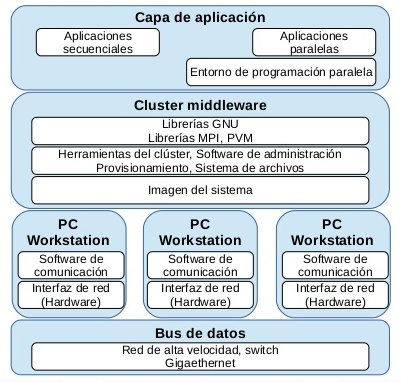
\includegraphics[scale=0.7]{graphics/clusterDef}
\end{figure}

La tecnología de clústeres es usada en tareas de cómputos o supercómputos, en servidores web y comercio electrónico y en bases de datos de alta disponibilidad. Es decir, las características de que se esperan de un clúster son las siguientes \cite{cluster}:

\begin{itemize}
\item \textbf{Alto rendimiento:} Debido a que se trata de un conjunto de ordenadores, la suma de su potencia hace que sean óptimos para tareas que requieran gran capacidad de computación y sean paralelizables. 

\item \textbf{Alta disponibilidad:} Por la misma razón, los clústeres deben ofrecer una rápida capacidad de recuperación ante fallos, por ejemplo, pudiendo recuperar los datos de un nodo perdido al guardar copias en otros o evitando la caída del sistema por el fallo en un nodo, siendo este sustituido.

\item \textbf{Balanceo de carga:} Un clúster debe distribuir el trabajo entre todos los nodos de la manera más equilibrada posible.

\item \textbf{Escalabilidad:} El sistema tendría que tener facilidad para adaptarse a las diferentes situaciones, siendo posible añadir o reducir capacidad del sistema mediante la adición o extracción de nodos del mismo.
\end{itemize}

Los elementos de un clúster son:

\begin{itemize}
\item \textbf{Bus de datos:} Que conecta a los nodos del clúster y permite la comunicación entre ellos.

\item \textbf{Nodos:} Es el conjunto de máquinas que forman el clúster, todas ellas tendrán que estar conectadas a la red y disponer de un software, el \gls{SO} que deberá ser multiproceso y multiusuario.

\item \textbf{Middleware:} Que permitirá el entendimiento entre las aplicaciones y el sistema operativo de los nodos. Es el encargado de hacer que el clúster sea visto por el usuario como una única entidad y, por otro lado, es el encargado de realizar el balanceo de tareas y permitir la escalabilidad del sistema.
\end{itemize}

\clearpage
\section{Infraestructura}
\subsection{Apache Spark \label{sparkEA}}
\textit{Apache Spark} \cite{spark} es un \gls{framework} de código abierto que permite el procesamiento de datos mediante la computación distribuida. Desarrollado originalmente por el departamento AMPLab de la Universidad de California, fue, posteriormente, donado a la fundación Apache, que lo ha mantenido desde entonces. 

Desarrollado en Scala \cite{scala} y con soporte para Java, Python y R, \textit{Apache Spark} proporciona una \gls{API} para programar clúster con paralelismo de datos implícito y tolerancia a fallos. Esta \gls{API} se apoya en la estructura llamada \gls{RDD}, donde se almacenan los datos particionados para permitir transformaciones en paralelo y que mantiene el índice de estas transformaciones para rehacerlas en caso de error.

Una buena característica de este \gls{framework} es el amplio soporte para la mayoría de los formatos de ficheros de datos, teniendo, además, integraciones con varios sistemas de almacenamiento como \gls{HDFS}, \textit{Apache Cassandra} \cite{cassandra} o Amazon S3 \cite{aws}. En la figura \ref{partSpark} podemos observar los diferentes componentes que conforman \textit{Apache Spark}.

\begin{figure}[htp!]
	\centering
	\caption{Componentes de \textit{Apache Spark} \cite{partsSpark}}
	\label{partSpark}
	\vspace{5pt}
	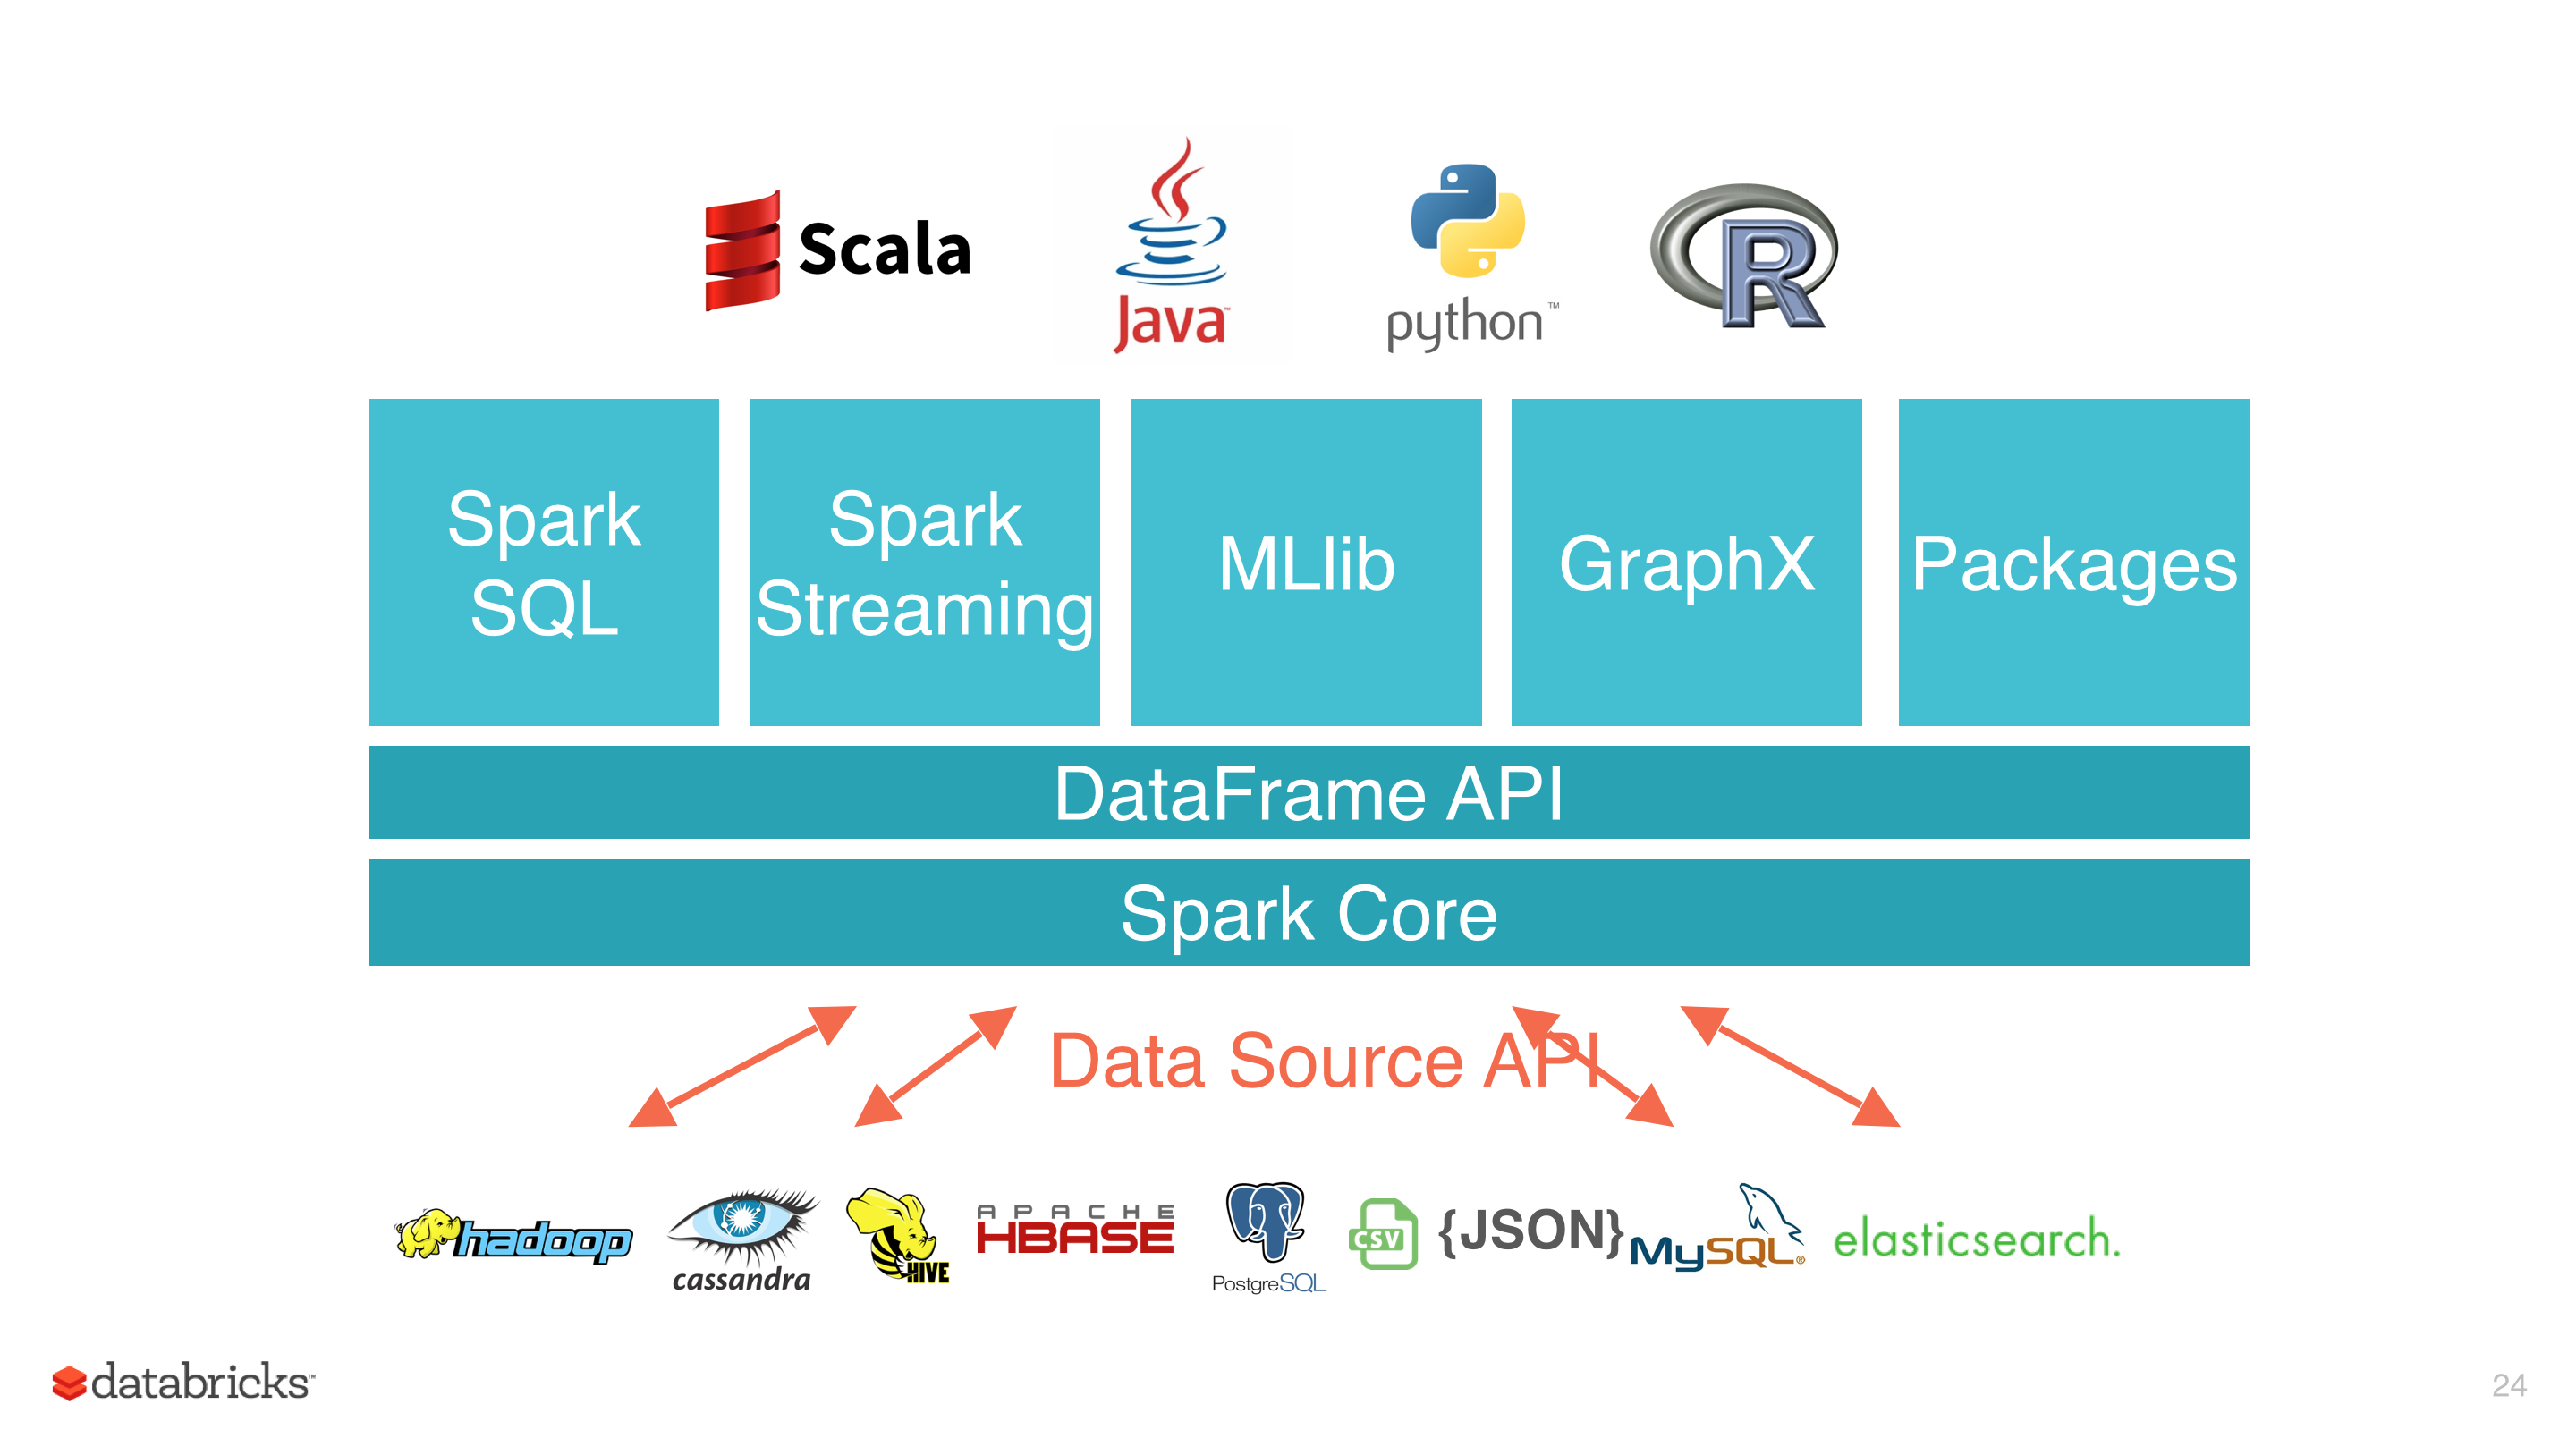
\includegraphics[scale=0.31]{graphics/partSpark}
\end{figure}

El \gls{framework} está formado por una base, sobre la que trabajan las diferentes librerías y paquetes del mismo. Dicha base está formada por el núcleo del programa, donde se crean y manipulan los \gls{RDD}, y la DataFrame API, que es una abstracción a más alto nivel de los \gls{RDD}, para simplificar su manipulación por el usuario.

Además \textit{Apache Spark} cuenta con diversas librerías como Spark SQL, para realizar consultas sobre los datos, Spark Streaming, para permitir la introducción y análisis de datos en tiempo real, MLib, para realizar aprendizaje automático, y Graphx, que permite la computación de grafos.

\subsubsection{Funcionamiento}
\textit{Apache Spark} basa su funcionamiento en dos conceptos, \gls{RDD} y \gls{DAG}. Una aplicación consiste en un controlador, llamado \textit{SparkContext}, que utiliza el código de usuario para crear y transformar \gls{RDD} y alcanzar el objetivo final. Estas transformaciones de los \gls{RDD}s son traducidos a gráficos \gls{DAG} para ser enviados al planificador y que este reparta las tareas.

\begin{figure}[htp!]
	\centering
	\caption{Funcionamiento de \textit{Apache Spark} \cite{partsSpark}}
	\label{sparkWork}
	\vspace{5pt}
	\includegraphics[scale=0.35]{graphics/sparkWork}
\end{figure}

\paragraph{\gls{RDD}: Resilient Distributed Dataset}
Esta será la solución utilizada en \textit{Apache Spark} para tratar los datos de una forma paralela y a prueba de errores. Además ofrece diferentes \gls{API}s para realizar transformaciones sobre los datos y permite el control sobre el modo de particionar los datos y el caché de los mismos.

Un \gls{RDD} puede ser creado a partir de un fichero en un almacenamiento externo o a partir de otro \gls{RDD} y es un sistema vago (\textit{lazy}), es decir, se guardan las operaciones que se realizarán sobre los datos, pero estas no son ejecutadas hasta que no se realiza la evaluación de los datos. Este sistema también es utilizado para la evitar los errores, donde el sistema sigue los pasos realizados desde el inicio para recomponer los datos correctamente.

Existen diferentes grupos de operaciones que se pueden realizar sobre un \gls{RDD}, estos son:

\begin{itemize}
\item \textbf{Transformaciones:} Permite realizar las funciones codificadas por el usuario sobre todos los datos del sistema, permite operaciones de agrupación, ordenamiento y particionamiento del \gls{RDD}. Estas operaciones son reflejadas en el grafo \gls{DAG}.

\item \textbf{Acciones:} Son las que inician el trabajo, es decir, hacen que se ejecuten las transformaciones estables

\item \textbf{Persistencia:} Permiten almacenar el \gls{RDD} en memoria o en disco de forma explicita.
\end{itemize}

\paragraph{\gls{DAG}: Direct Acyclic Graph} 
Es la forma de codificación de los trabajos sobre los \gls{RDD}s utilizada en \textit{Apache Spark}. Indica el flujo que seguirá la aplicación durante la ejecución que, generalmente, se basa en leer los datos del origen, realizar las transformaciones oportunas y materializar los datos obtenidos.

\begin{figure}[htp!]
	\centering
	\caption{Transformaciones sobre un \gls{RDD} representadas en un \gls{DAG} \cite{partsSpark}}
	\label{dag}
	\vspace{5pt}
	\includegraphics[scale=0.4]{graphics/dag}
\end{figure}

Este componente también es el que se encarga de establecer las diferentes tareas del trabajo que, posteriormente, serán repartidas entre los nodos del clúster para paralelizar el trabajo.

Una de las características que diferencia \textit{Apache Spark} es la forma en la que gestiona los datos, este \gls{framework} guarda los datos en la memoria \gls{RAM} del dispositivo, sin llegar escribir a disco, por lo que el acceso a estos es muy rápido. Por ello, hace que la velocidad en procesos iterativos, donde se consultan los mismos datos de forma continua, sea muy elevada, mejorando con creces los tiempos de otros sistemas como MapReduce \cite{compSpark}.

\begin{figure}[htp!]
	\centering
	\caption{\gls{RDD} distribuido en diferentes máquinas \cite{sparkbook}}
	\label{rdddistribuido}
	\vspace{5pt}
	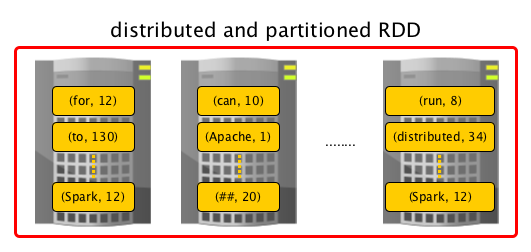
\includegraphics[scale=0.6]{graphics/rdddistribuido}
\end{figure}

\subsubsection{Librerías}
Como se ha indicado anteriormente, \textit{Apache Spark} incluye diferentes librerías que trabajan sobre la base del \gls{framework}. Estas son:

\begin{itemize}
\item \textbf{Spark SQL:} Permite el soporte para datos estructurados o semi-estructurados para realizar consultas \gls{SQL} sobre ellos. Estos datos pueden ser modificados con funciones específicas de \textit{Apache Spark} o mediante el lenguaje \gls{SQL}.

\item \textbf{Spark Streaming:} Permite el análisis en tiempo real de datos mediante la introducción de estos en mini lotes de datos. Este sistema aunque cumple su función no es tan potente como el ofrecido por otras alternativas como \textit{Apache Flink} \cite{flink} o \textit{Apache Storm} \cite{storm}.

\item \textbf{MLib:} Es un \gls{framework} de aprendizaje automático distribuido. Este permite diferente tipos de análisis sobre los datos: clasificaciones, regresiones, clusterizaciones, optimizaciones, etc.

\item \textbf{GraphX:} Es un procesador de grafos distribuido. Es muy veloz para grafos que no tienen que ser actualizados, sin embargo, debido a la naturaleza inmutable de los \gls{RDD} no es una herramienta válida para grafos que se modifiquen.
\end{itemize}

\subsection{Apache Hadoop}
\textit{Apache Hadoop} \cite{hadoop} es otro \gls{framework} de código abierto que permite el tratamiento de grandes cantidades de datos de forma distribuida. Desarrollado en Java, permite la gestión de clústeres de un nodo hasta cientos de ellos de forma sencilla. Al establecer sistemas distribuidos estos tienen una alta tolerancia a los fallos.

\textit{Apache Hadoop} cuenta con cuatro módulos principales, aunque cuenta con muchos más proyectos totalmente compatibles: 

\begin{itemize}
\item \textbf{Hadoop Common:} Utilidades comunes que soportan el resto de módulos.

\item \textbf{Hadoop Distributed File System (\gls{HDFS})} Sistema de ficheros distribuido que permite la replicación de los datos en los nodos del sistema.

\item \textbf{Hadoop YARN:} Es un \gls{framework} que se encarga de la gestión de los trabajos y los recursos del clúster.

\item \textbf{Hadoop Mapreduce:} Sistema basado en YARN para el procesamiento paralelo de grandes cantidades de datos.
\end{itemize}

En este proyecto, debido a que utilizamos \textit{Apache Spark} para la gestión del clúster, no utilizaremos la mayoría de los módulos de \textit{Apache Hadoop}. El módulo que se utilizará será el sistema de ficheros \gls{HDFS} por la configuración distribuida del clúster doméstico. 

Con este sistema realizaremos la replicación de los ficheros de datos en los diferentes nodos del sistema y, de esa forma, ahorrar la transmisión de estos durante la ejecución de los trabajos y, así, mejorar los tiempos de procesamiento.

\subsubsection{Hadoop Distributed File System (\gls{HDFS})}
\gls{HDFS} es un sistema de ficheros distribuido, escalable y portable escrito en Java. Este permite el almacenado de grandes cantidades de datos mediante la distribución de estos en diferentes máquinas. \gls{HDFS} es muy tolerante a los fallos y esta diseñado para correr en hardware de bajo coste. 

\gls{HDFS} fue construido con las siguientes asunciones y objetivos:

\begin{itemize}
\item \textbf{Errores de hardware:} Los fallos de hardware son más una norma que una excepción en la realidad, por ello, \gls{HDFS} es muy tolerante a los fallos, distribuyendo y replicando los datos en diferentes máquinas del clúster para no perder el acceso a ellos por la caída de algún nodo.

\item \textbf{Acceso al streaming de datos:} \gls{HDFS} fue concebido para aplicaciones que necesitan un buen rendimiento en el acceso a los datos, más que para su manipulación continua por los usuarios. Por ello, se centra más en el procesamiento en lotes.

\item \textbf{Grandes volúmenes de datos:} \gls{HDFS} está afinado para manejar ficheros de datos que van desde los cientos de gigasbytes hasta terabytes de tamaño.

\item \textbf{Modelo de coherencia simple:} Las aplicaciones que usan este sistema necesitan el acceso a la lectura del fichero más que sus modificaciones. Por ello, el sistema del \gls{HDFS} usa un modelo ``escribe una vez y lee el resto'', por lo que una vez que se crea un fichero, se escribe y guarda, este no vuelve a modificarse excepto para reducir la cantidad de datos o añadir más.

\item \textbf{``Mover la capacidad de computación es más barato que mover los datos'':} Una aplicación es más eficiente si la computación se realiza cerca de los datos, ya que ahorras el tiempo de transporte de estos. Esta es la premisa que sigue \gls{HDFS} y por ello se replican los datos en todos los sistemas para realizar las operaciones sobre estos en los propios nodos.

\item \textbf{``Portabilidad entre hardware y software heterogéneo: } \gls{HDFS} ha sido diseñado para ser fácilmente portado entre sistemas y plataformas.
\end{itemize}

\begin{figure}[htp!]
	\centering
	\caption{Arquitectura del \gls{HDFS} \cite{hadoop}}
	\label{hdfsarchitecture}
	\vspace{5pt}
	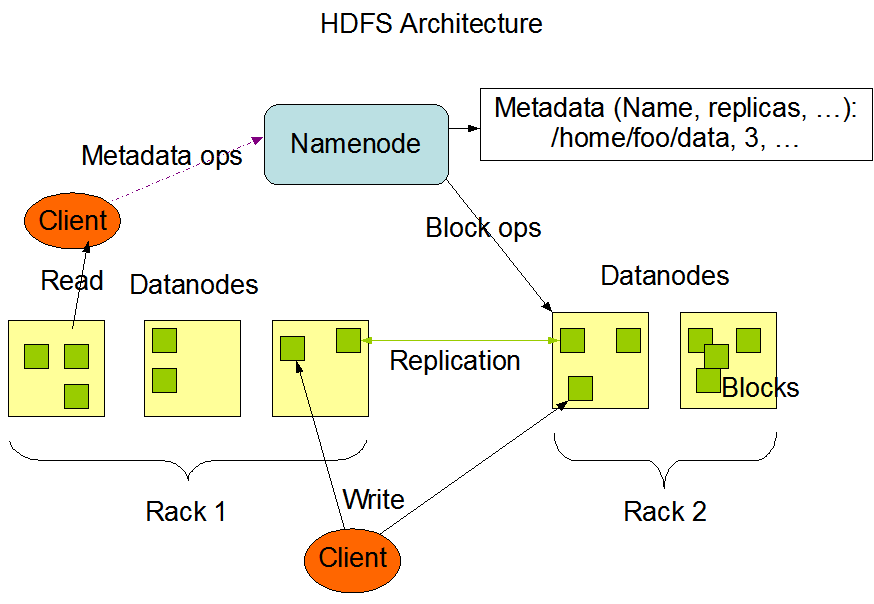
\includegraphics[scale=0.6]{graphics/hdfsarchitecture}
\end{figure}

En la figura \ref{hdfsarchitecture} podemos ver la arquitectura de un sistema \gls{HDFS}, este esta basado en la estructura maestro/esclavo, donde existe una \textit{Namenode} que hace de maestro y gestiona el sistema de ficheros y regula el acceso a los ficheros por los clientes. Por otro lado, están los \textit{Datanodes}, uno por nodo, que es donde se almacenan y gestionan los datos del sistema.

Por otro lado, dentro de estos \textit{Datanodes} encontramos los bloques, que son partes o fragmentos de los datos originales y que se replican por los diferentes nodos.

\subsection{Apache Parquet \label{parquetBeneficios}}
\textit{Apache Parquet} es un formato de fichero de código abierto basado en el almacenamiento columnar. Este es compatible con la mayoría de los \gls{framework}s del ecosistema Hadoop y con \textit{Apache Spark} y ofrece sistemas de compresión y codificación eficientes para mejorar su eficiencia.

\begin{figure}[htp!]
	\centering
	\caption{Comparación entre almacenamiento columnar y basado en filas \cite{column}}
	\label{column}
	\vspace{5pt}
	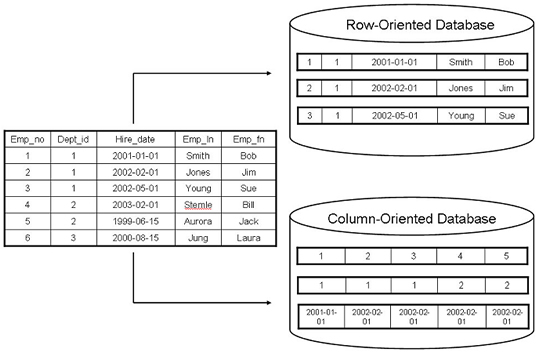
\includegraphics[scale=0.7]{graphics/column}
\end{figure}

El almacenamiento columnar es un modelo en el que la tabla se guarda por columnas en vez de por filas, es decir, lo que se guarda es el conjunto de los datos de una columna y se establece una identificación para saber a que elemento pertenecen los datos. Este modelo es más rápido en muchos casos ya que se puede acceder directamente al atributo deseado, sin tener que descartar el resto de la fila \cite{column}.

Por otro lado, este tipo de almacenamiento es mejor en cuanto al ahorro de espacio debido a que su estructura es más fácil de comprimir, por ejemplo, no es necesario indicar el tipo de cada valor, ya que son todos del mismo tipo al tratarse de la misma columna de la tabla. 

Otra ventaja se aporta cuando los valores de la columna se repiten, ya que este se guarda una vez y se establece las posiciones en las que ocurre. También usa una codificación mínima para los enteros pequeños y permite el trabajo de los datos con aplicaciones de vectorización.

\begin{figure}[htp!]
	\centering
	\caption{Espacio ocupado en disco de un archivo por diferentes formatos \cite{parquetSpace}}
	\label{parquetSpace}
	\vspace{5pt}
	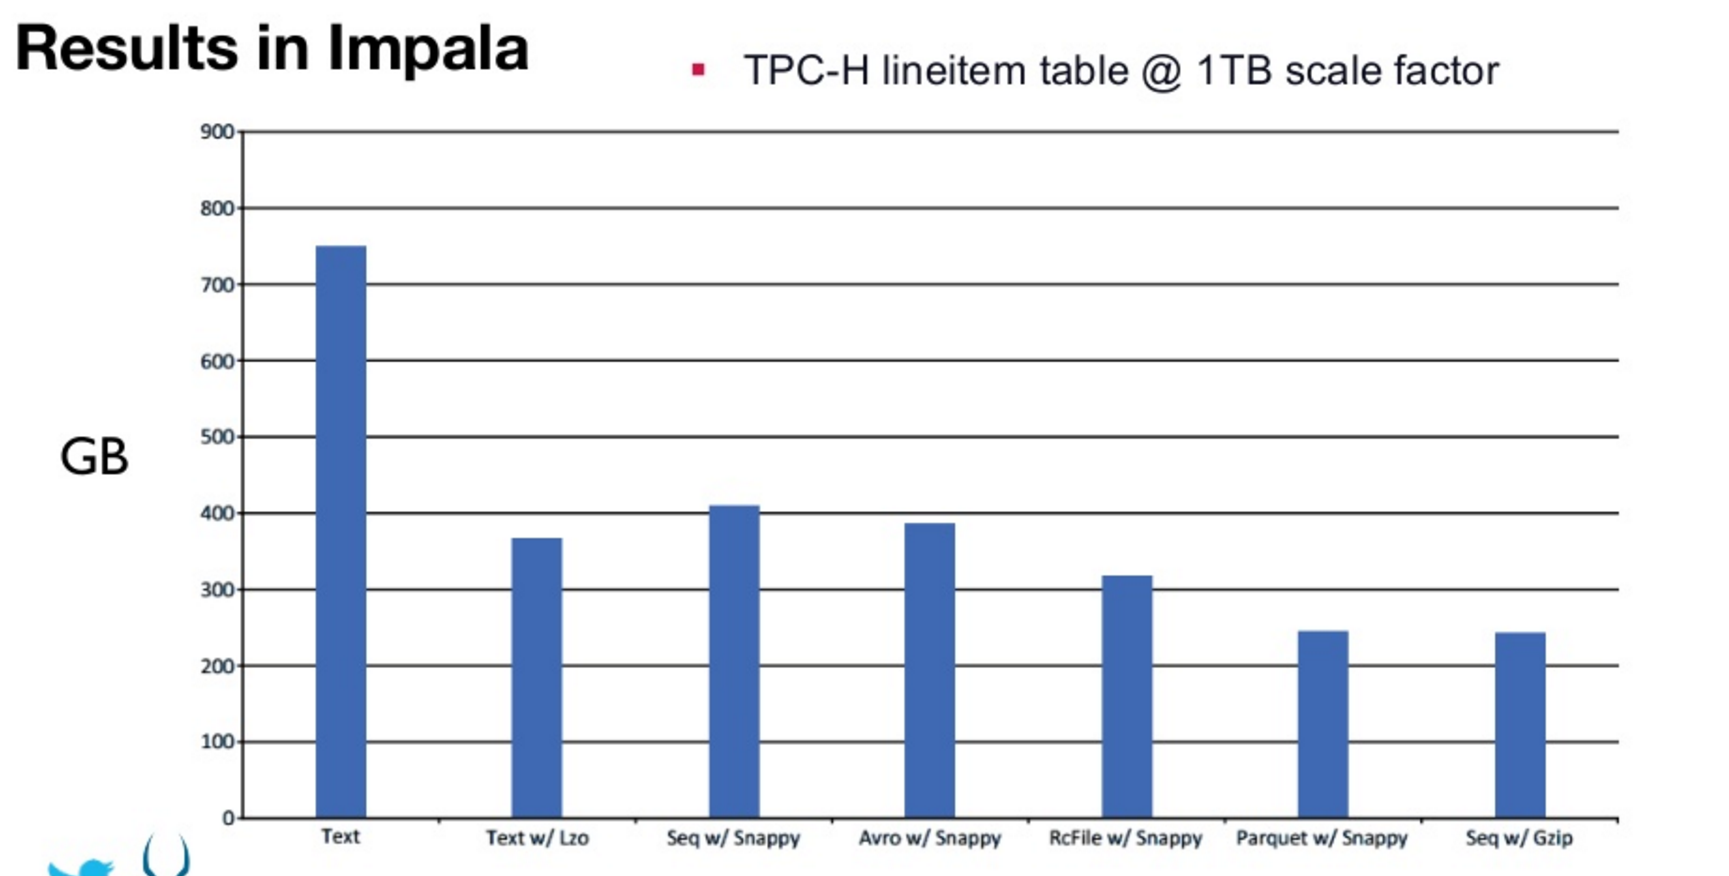
\includegraphics[scale=0.2]{graphics/parquetSpace}
\end{figure}

En este caso, para la compresión de los ficheros de \textit{Apache Parquet} utilizaremos la librería \textit{Snappy} \cite{snappyLib}, que es compatible con este formato. \textit{Snappy} es una librería de compresión y descompresión creada por Google cuya intención no es conseguir el mínimo tamaño de fichero, si no la mayor velocidad de compresión y descompresión.